\documentclass{dsekprotokoll}

\usepackage[T1]{fontenc}
\usepackage[utf8]{inputenc}
\usepackage[swedish]{babel}
\usepackage{tikz}
\usetikzlibrary{arrows.meta,positioning}

\setheader{Policy för Ekonomirutiner}{Policydokument}{}

\title{Policy för Ekonomirutiner}
\author{Joel Bäcker, Sean Jentz}

\begin{document}
\maketitle
\section{Formalia}
\subsection{Sammanfattning}
Policyn beskriver vilka rutiner finns vid hantering av sektionens ekonomi och hur attesteringsrätten fungerar.
\subsection{Syfte}
D-sektionen är en ideell förening och har inget vinstintresse. Därmed skall ingen funktionär inom D-sektionen behöva betala pengar ur egen ficka för att kunna utföra sitt uppdrag så som uppdraget är beskrivet i reglementet. Ingen funktionär ska tjäna pengar på sektionens verksamhet.

\par Denna policy beskriver D-sektionen syn på ekonomirutiner och attesteringsrätt. Syftet är att ge styrelsen såväl som funktionärer vägledning i frågor gällande kontanthantering, utlägg samt attest.
\subsection{Omfattning}
Sektionen i sin helhet.
\subsection{Ägande}
Sektionsmötet äger policyn.
\subsection{Historik}
Ursprungligen antagen enligt beslut: VTM/2017
Omarbetning fastställd enligt beslut (samt motionär):
\begin{itemize}
\item VTM 2021 (Joel Bäcker \& Sean Jentz)
\item VTM 2022 (Emma Kujala)
\end{itemize}
Uppdaterad enl. Policy för Policyer på HTM2 2021.

% vad som ska vara med 

% interna transaktioner 
% hur mycket kan man köpa för på olika möten
% utlägg som går utanför rambudget
% attestering av projektgrupp, medalj, trivsel, valberedningen

% donationer
% värdepapper

\section{Terminologi}
\begin{description}
\item[Budgetpost] En budgetpost visar hur mycket sektionen har budgeterat för en viss kostnad eller vinst. Till exempel är Mötesfika en budgetpost.
\item[Kostnadsställe] Ett kostnadsställe består av budgetposter för både kostnader och vinster för en viss del av en resultatenhets verksamhet. Varje kostnadsställe har en egen kod, till exempel är SEKT01 ett kostnadsställe inom resultatenheten Sektion.
\item[Resultatenhet] Varje utskott, samt Styrelsen och Sektionen är sin egen resultatenhet. Resultatenheten är uppdelad i ett eller flera kostnadsställen.
\item[Rambudget] Rambudgeten är den budgeten som ägs av sektionsmötet. Det är en sammanställning av alla resultatenheter och deras kostnadsställen. 
\end{description}

\section{Avtal}
Firmatecknare äger alltid rätt att besluta om avtal då det innebär ett
positivt nettoresultat samt avtal som följer redan lagd budget. En förutsättning är att avtal
inte går emot D-sektionen eller Teknologkårens styrdokument.

\section{Utlägg}
Nedan följer punkter som sektionsmedlemmar ska följa vid utlägg.

\begin{itemize}
    \item utläggs- och intäktsräkningar skall skyndsamt lämnas in till Skattmästeriet om ej särskilda skäl finns.

    \item utlägg större än 1000 SEK som direkt medverkar till större budgetavsteg och/eller inte direkt kan kopplas till daglig verksamhet ska först godkännas på ett styrelsemöte/sektionsmöte. Styrelsemötet/sektionsmötet äger tolkningsrätt i vad som anses vara daglig verksamhet. Beslut tagna på styrelsemöte angående sådana utlägg skall redogöras på sektionsmöte.

    \item alla köp i sektionens namn ska redogöras genom en utläggsräkning tillsammans med ett fysiskt kvitto, kontoutdrag räknas inte.
\end{itemize}

\section{Kontanthantering}
Nedan följer punkter som sektionsmedlemmar ska följa vid kontanthantering.
\begin{itemize}
    \item Sektionen ska eftersträva minimal kontanthantering och istället jobba med digitala betalningsalternativ.
    \item kontantbelopp som överstiger 3000 kronor skall och måste räknas av minst två personer.
\end{itemize}

\section{Attest}
Detta avsnitt ämnar att klargöra kring attest kring personliga utlägg samt köp gjort med sektionskort.

\subsection{Rutiner}
\begin{itemize}
    \item samtliga utlägg skall signeras av två individer, personen som gjort utlägget och en som godkänner utlägget. Godkännandet ska, om möjligt, utföras av individ från den närmst följande instansen enligt diagram nedan.
    \item utlägg kan inte godkännas av samma individ som gjort utlägget.
    \item en högre instans kan i samtliga fall ersätta en lägre instans signatur om så behövs. En lägre instans kan aldrig godkänna en högre instans utlägg.
    \item en individ signerar alltid i egenskap av sin högsta instans.
\end{itemize}

\subsection{Attesträtt}
Nedan följer hur attesteringsrätt fungerar för mästare, vice skattmästare och firmatecknare. Attestskall alltid sträva efter att skötas på lägsta möjliga instans. Diagrammet nedan är endast för vägledning, nedanstående punkter beskriver mer exakta bestämmelser. Således har inte godtycklig styrelseledamot attesteringsrätt för Teknikfokusansvarig eller utedishoansvarig även fast diagrammet antyder detta.

Utskott som inte har en utskottsordförande som inte sitter i styrelsen vänder sig till firmatecknare för att få sina utlägg attesterade.

\begin{itemize}
    \item \textbf{Firmatecknare} äger attesteringsrätt för alla utlägg och kan attesteras av varandra. Firmatecknare kan inte attestera sina egna utlägg.
    \item \textbf{Vice skattmästare} äger attesteringsrätt för alla utlägg gjorda av funktionär. Vice skattmästare kan inte attestera styrelseledamöter.
    \item \textbf{Näringslivsansvarig} äger attesteringsrätt för alla utlägg gjorda för näringslivsutskottet, där även utlägg gjorda av Teknikfokusansvarig.
    \item \textbf{Aktivitetsansvarig} äger attesteringsrätt för alla utlägg gjorda för aktivitetsutskottet, där även utedischoansvarig.
    \item \textbf{Övriga styrelseledamöter} äger attersteringsrätt för utskott för vilka dem är utskottsordförande, förutom Vice Ordförande som inte har någon attesteringsrätt.
    \item \textbf{Teknikfokusansvarig} äger attesteringsrätt för alla utlägg gjorda för teknikfokus.
\end{itemize}
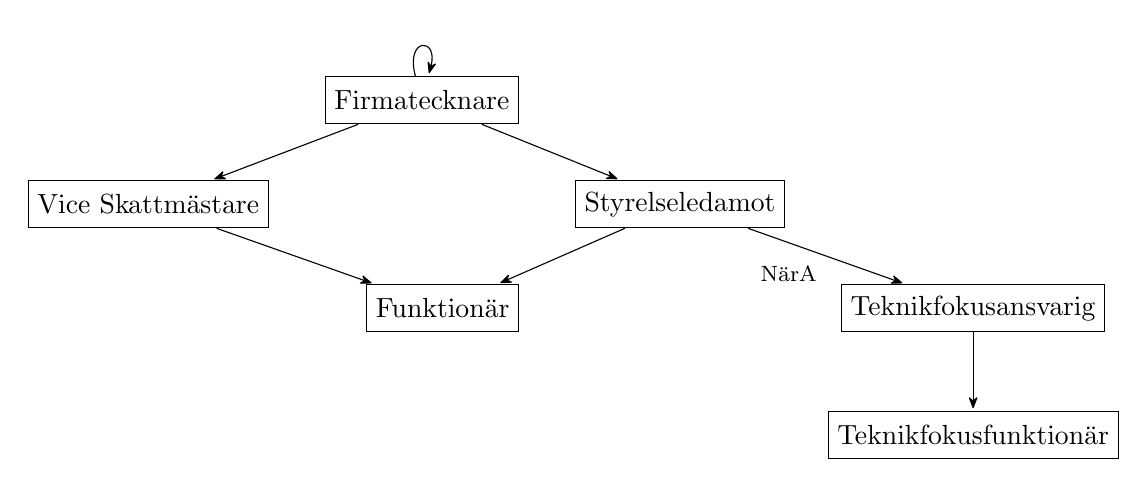
\begin{tikzpicture}
  [shorten >=1pt,
   node distance=1cm,
%% on grid,
   >={Stealth[round]},
   squarednode/.style={rectangle,
                      draw=black,
                      minimum size=6mm},]
  \node[squarednode] (ft)                           {Firmatecknare};
  \node[squarednode] (vice)   [below left =of ft]   {Vice Skattmästare};
  \node[squarednode] (styr)   [below right=of ft]   {Styrelseledamot};
  \node[squarednode] (funk)   [below left =of styr] {Funktionär};
  \node[squarednode] (tekf)   [below right=of styr] {Teknikfokusansvarig};
  \node[squarednode] (tekf-f) [below=of tekf]       {Teknikfokusfunktionär};
  \path[->,every node/.style={font=\footnotesize}]
  (ft)   edge [loop above] node               {}     ()
         edge              node [below left ] {}     (vice)
         edge              node [below right] {}     (styr)
  (vice) edge              node [below right] {}     (funk)
  (styr) edge              node [below left ] {}     (funk)
         edge              node [below left ] {NärA} (tekf)
  (tekf) edge              node [below]       {}     (tekf-f);
\end{tikzpicture}

\section{Betalkort}
Sektionen äger ett antal betalkort, ofta kallat Sektionskort, som ska användas för betalning i sektionens namn. Dessa betalkort skall användas för att minimera behovet av privata utlägg.

Poster som erhåller ett betalkort avgörs av styrelsen.

\section{Budgetavsteg}
Om en budgetpost inom en resultatenhet, hela resultatenheten eller rambudgeten i sin helhet avsiktligt beräknas avvika negativt kan ett budgetavsteg göras.

\subsection{Riktlinjer}
\begin{itemize}
  \item Styrelsemöte får besluta om att höja kostnader i ett kostnadsställe om denna kostnaden täcks av en inkomst inom samma resultatenhet.
  \item Styrelsemöte kan fatta beslut om budgetavsteg för belopp mindre än 50\% upp till 10000 SEK per resultatenhet.
  \item På ett sektionsmöte finns inga begränsningar på vilka budgetförändringar som kan ske.
\end{itemize}

\subsection{Redovisning av budgetavsteg}
Budgetavsteg gjorda av styrelsen måste redovisas på nästkommande sektionsmöte.

\section{Donationer}
\subsection{Inkomna Donationer}
Vid inkomna donationer ska dessa pengar öronmärkas för ett specifik ändamål samt läggas i lämplig fond. I de fall där inget specifikt ändamål angetts hanteras de som om det inte fanns en specifik fond och behöver således inte heller öronmärkas till något speciellt.

Styrelsen kan ta emot och disponera donationer upp till 10000 SEK men högre än så måste ett sektionsmötesbeslut avgöra hur man ska disponera pengarna.

\subsection{Utgående Donationer}
Vid försäljning av varor kan ett utskott välja att ta emot donationer som ska gå till olika icke-vinst drivande, ideella, välgörenhetsorganisationer. Dessa pengar ska inte användas av något annat än till dessa ändamål. Styrelsemöte avgör organisationens lämplighet.

\end{document}
